%update: Nov 21 citation done , figure done. 
%update: Nov 10 by zc, add more text(slightly edited), uploaded and compiled all figures. 
%update: Nov 09 by professor, rewrite the first half of text. 

\begin{savequote}[75mm] 
I am somewhat exhausted; I wonder how a battery feels when it pours electricity into a non-conductor?
\qauthor{Sherlock Holmes (Arthur Conan Doyle)} 
\end{savequote}

\chapter{\emph{In situ} TEM electrical probing for ultrastable sodium ion batteries}

\newthought{Sodium-ion batteries (SIBs)}, as an important alternative for future energy storage, have been on stage since 1980s. Among many anode materials, elemental phosphorus (P) has attracted most of the interest in recent years because of  large theoretical capacity, i.e. 2596 $mAh/g$. The prime disadvantage, however, of a P anode is its poor conductivity and fast structural degradation due to volume expansion, as much as $>$490$\%$, over working cycles. To address this issue, I redesigned the anode structure via fabricating a flexible paper made of amorphous P and N-doped graphene. The as-fabricated anode delivers ultrastable characteristics and superb rate capability, 809 $mAh/g$ at 1500 $mA/g$. The extraordinary structural integrity of this new anode was then studied via \emph{in situ} experiments inside a high-resolution transmission electron microscope (HRTEM), thereby the cyclic dynamics and sodiation/desodiation mechanisms were thoroughly understood. To confirm my experimental results, Density Functional Theory (DFT) calculations were additionally performed to indeed confirm that the N-doped graphene contributes to an increase in capacity for Na storage, and to an improved anode rate performance.

\section{Introduction}
Sodium ion batteries (SIBs) are receiving considerable attention and have bright expectations as one of the most promising alternatives to lithium ion batteries (LIBs) for energy storage.\cite{Ren2014c,Yang2011c,Liu2014a,Wen2014b,Shen2015b,wang2014e,Wu2014b,Yao2015b,Ni2014b} Both battery types possess analogous chemistry, but SIBs are cheaper because of more abundant sodium natural resources. In the recent reports, the cathode performance in SIBs was found to be comparable with that of the LIBs.\cite{Sun2014b,Barpanda2014b} However, such performance is still the major constraint for the immediate practical applications. There have been an increasing interest in developing high-power and high-capacity anode materials for the next generation SIBs,\cite{Ong2011b,Palomares2012b,Zhu2014b,Yu2014b,Berthelot2011b,Qian2012d,Wang2013g,Komaba2011b,Cao2012b,Wang2013h,Xu2013b,Qian2012e} such as transition metal oxides,\cite{Zhu2014b,Yu2014b,Berthelot2011b} Prussian blue analogues,\cite{Qian2012d,Wang2013g} hard carbon materials,\cite{Komaba2011b}, nanowires,\cite{Cao2012b} graphene,\cite{Wen2014b,Wang2013h}, tin composite, \cite{Xu2013b} and antimony-based materials,\cite{Qian2012e} but their specific capacities are still not competitive for future applications(<800 mAh/g). \\

\begin{figure}  
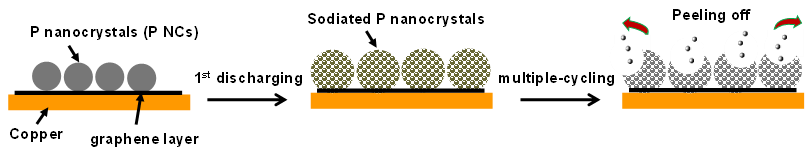
\includegraphics[width=\textwidth]{figures/figure4_s1}
\caption[Peeling off after cycling]
{Schematic diagram of the structural fracture of a high-volume-change type P anode, in which P nanocrystals anchored on the graphene layer are placed on the surface of a Cu current collector. After 1st discharging, there is a large volumetric expansion (>200-500\%) for P NCs; during cycling, such large volume change will lead to the pulverization and thus peeling off the electrode.
\label{fig:4_s1}}
\end{figure}

Among the hottest materials, elemental phosphorus (P) is one of the most attractive candidates with an ultra-high theoretical capacity of 2596 mAh/g,\cite{Qian2013b,Kim2013c,Li2013c} i.e. about 7 times higher than that of the commercial graphite anode in LIBs. The key challenge associated with a phosphorus anode is its rapid structural degradation caused by huge volume change (>490\%) under cycling. For conventional crystalline phosphorus (Figure \ref{fig:4_s1}), upon Na insertion, the P crystals are pulverized and thus the electrode film surface cracks (as a result of ~200-500\% volumetric expansion), leading to phosphorous peeling off from the current collector, which, in turn, gives a significant performance fading. So, stabilizing or sustaining the rigidness of the phosphorus anode structure during cycling is the practical key toward the improvement of the cycling performance of a P-based SIB anode. Very recently, notable breakthroughs have been witnessed in stabilizing anode structure through a design of amorphous P/carbon hybrids.\cite{Qian2013b,Kim2013c,Li2013c} For example, Qian et al. reported that the amorphous P/C hybrids prepared under high-energy mechanical milling had demonstrated a considerable capacity retention of 68\% after 60 cycles at the current density of 250 mA/g.\cite{Qian2013b} Kim et al. demonstrated that a similar amorphous P/C structure is able to deliver as high as 80\% reversible capacity and less than 7\% capacity fading after 30 cycles at a current density of 143 mA/g.\cite{Kim2013c} In addition, Chou et al. fabricated a composite anode via simple hand-grinding of commercial microsized red phosphorus and carbon nanotubes (CNTs); this demonstrated a high capacity retention of 76.6\% over 10 cycles.\cite{Li2013c} The improvements in cycling stability in the regarded reports were indeed remarkable, however, capacity retentions of less than 80\% still indicate that further developments are still needed in order to meet the practical requirements.\cite{Luo2015b}\\

\begin{figure}  
\centering
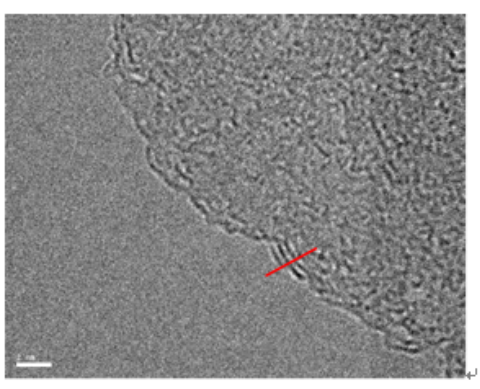
\includegraphics[width=300pt]{figures/figure4_s2}
\caption[TEM of GN]
{HRTEM image of an N-doped graphene (GN).
\label{fig:4_s2}}
\end{figure}

\begin{figure}  
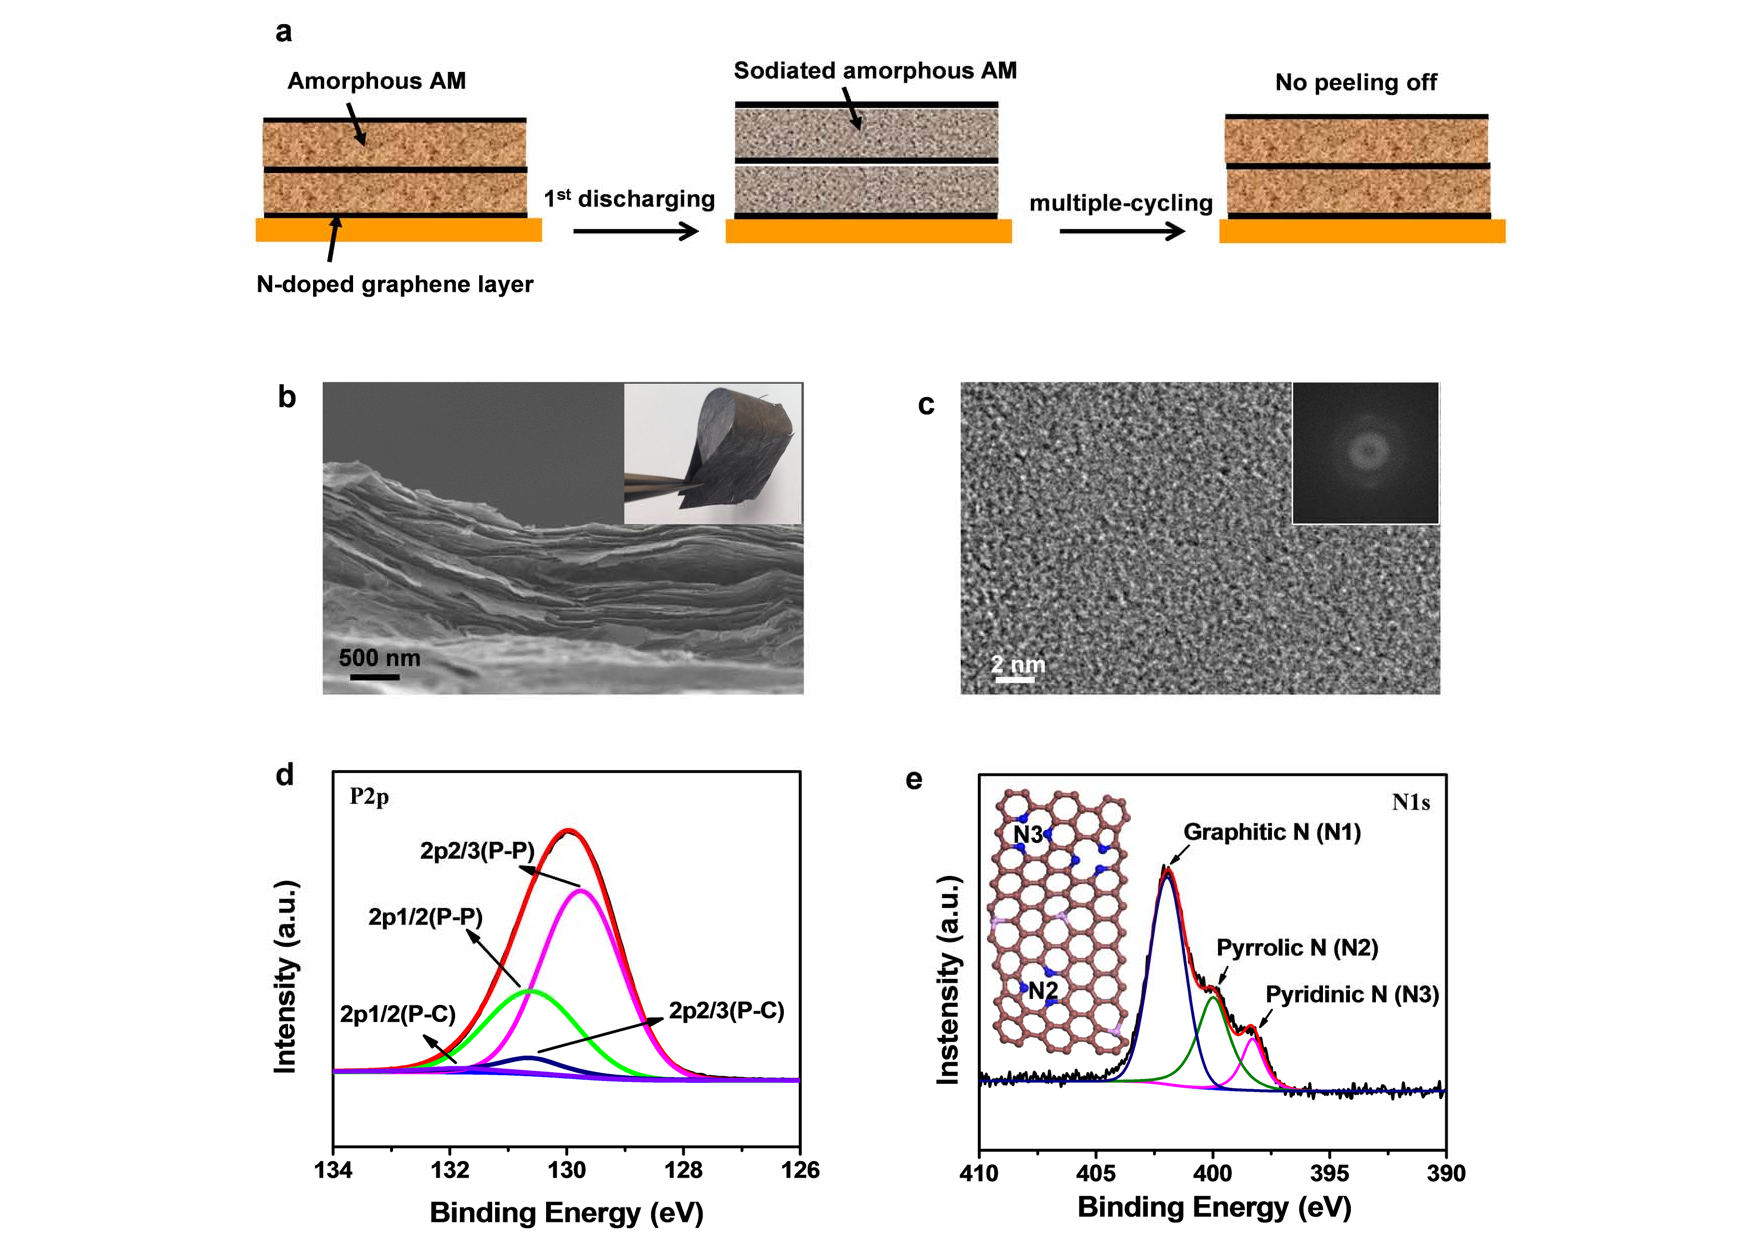
\includegraphics[width=320pt, angle=-90]{figures/figure4_1}
\caption[Layered structure design]
{(a) Illustrative scheme of the designed layered anode structure. (b) SEM image of the cross section of a P@GN paper, the inset shows its paperlike appearance. (c) HRTEM image and the corresponding FFT pattern of the P@GN portion confirming its amorphous structure. d-e) P2p and N1s XPS spectra of P@GN. N2 and N3 represent pyrrolic N and pyridinic N, respectively. 
\label{fig:4_1}}
\end{figure}

To obtain a stable P-based Na-ion battery anode having high capacity retention and rate performance, a flexible hybrid amorphous P-embedded N-doped graphene paper was designed and studied in my work. Unlike the standard methods which assemble the P and C components via any mechanical mixing (milling or grinding), a smarter design should tackle the existing problems, such as electrode chemical stability during sodiation-desodiation and mechanical robustness after hybridization. Therefore, a few-layered N-doped graphene (GN) (Figure \ref{fig:4_s2}) is herein selected as a substrate, whose two-dimensional (2D) nanosheet architecture provides a decent framework ensuring uniform deposition of amorphous P.\cite{Nicolosi2013b,Huang2015b} Several advantages associated with the designed amorphous P@GN hybrids (Figure \ref{fig:4_1}a) prepared by the developed so-called “phase-transformation” route are:\\
(1) Compared with crystalline P (Figure \ref{fig:4_s3}), amorphous P is more stable because of its relatively small volume change.\cite{Qian2013b,Kim2013c} Through the uniform confinement of the amorphous P within GN frameworks, the flexible GN can effectively buffer the volume change. This effectively prevents the electrode fracture and ensures the improvement of the battery capacity retention during electrochemical cycling;\\
(2) The possibly formed robust P-C bonds between P and GN layers anchor both components, serving like several elastic “springs” between them; this also helps to further enhance the stability of the anode;\\
(3) The GN nanosheets provide high conductivity electron transport networks and robust mechanical backbones, so that amorphous P could be very electrochemically active. In addition, the high tenacity of GN is useful to accommodate the volumetric expansion of P without mechanical damage or peeling off effects. Furthermore, N-doped graphene also contributes with a certain capacity to the SIBs and brings the fast sodium ion transport according to the DFT calculations.
Thus in this Chapter, I show that the above-mentioned three key features of the amorphous P@GN structure endows the large-volume-change anode with a superb capacity retention (>85\% over 350 cycles), outstanding cycle stability (0.002\% decay per cycle from 2nd to 350th cycle), and excellent rate capability (809 mAh/g at 1500 mA/g). Most importantly, state-of-the-art {\em in situ} probing experiments in HRTEM and supporting theoretical calculations finally uncover the key advantages of the present design and ensure the future developments of the P-based high-performance SIB anode structures, while getting deep insights into the associated atomistic mechanisms. 

\begin{figure}  
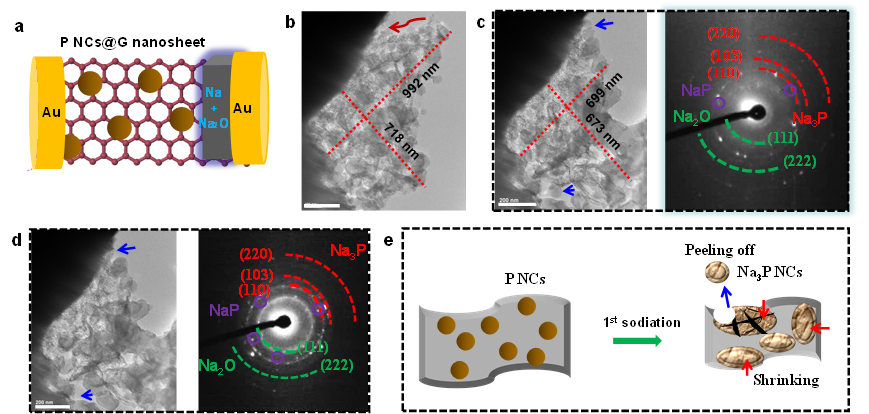
\includegraphics[width=320pt,angle=0]{figures/figure4_s3}
\caption[Layered structure design]
{a) Schematic illustration of an individual P nanocrystals@G (P NCs@G) nanosheet prototype sodium battery device fabricated under {\em in situ} TEM. b) TEM image of the nano-SIB at the initial stage. c-d) Time-dependent TEM images and SAED patterns of sodiated P NCs@G nanosheet upon sodiation at 5 s and 120 s. e) The schematic illustration of the 1st sodiation-desodiation process of P@GN nanosheet. Red arrows indicate the shrinkage, while blue arrows indicate particles peeled off. Scale bars: 200 nm. 
\label{fig:4_s3}}
\end{figure}

\section{Experimental}
%from main text.
Amorphous P@GN paper was prepared by a designed "phase-transformation" route. Bulk red P was heated to form P4 vapors in a sealed ampule, which were adsorbed and deposited within the inter-layers of GN; it changed back into amorphous red P after condensation.\cite{Roth1947b} Thus, a butter-bread-like structure composed of flexible conductive GN layers and thin amorphous red P layers between them was fabricated (Figure \ref{fig:4_1}b). 
%from SI.
Synthesis of P@GN. Graphene oxide (GO) suspension used in this work was prepared via a modified method. 50 mg of graphene oxide was loaded in a ceramic boat in a tube furnace followed by its heat treatment at 600 degrees Celsius for 1.5 hours in a gas mixture of NH3 and Ar (1:2 vol/vol) under a total flow rate of 150 ml/min. Commercial red phosphorus was dispersed in water and put into a Teflon-lined stainless autoclave. The autoclave was heated to 200 degrees Celsius and maintained for 12 h to remove surface oxides. As-prepared N-doped graphene (GN) products were properly mixed together with the pretreated red phosphorus powder, and sealed in an ampule in an inert Ar atmosphere. The sealed reactors were thermally treated at 500 degrees Celsius for 1 hour and then at 280 degrees Celsius for several hrs in the furnace, before natural cooling to room temperature. The final product was washed with CS2, water and methanol, and then dried at 60 degrees.\\

Characterization. TEM images were taken with a 300 kV JEOL 3000F microscope. Samples were first dispersed in ethanol and then collected using carbon-film-covered copper grids. To avoid possible electron beam effects (such as radiolysis or sputtering damage of both Na-containing species and graphene lattice) the beam intensity was minimized. Scanning electron microscopy (SEM) images were recorded on a Hitachi S4800 electron microscope operating at 15 kV. XRD patterns were taken on a Philips X Pert PRO MPD X-ray diffractometer operated at 35 kV and 45 mA with Cu Kα radiation. XPS measurements were carried out on an ESCALab220i-XL spectrometer by using a twin-anode Al Ka (1486.6 eV) X-ray source. All the spectra were calibrated to the binding energy of C 1s peak at 284.6 eV. The background pressure was ~3 x 10-7 Pa. Raman spectra were collected on a Horiba Jobin-Yoon T6400 Raman spectrometer.\\
Electrochemical tests: The electrochemical properties of P@GN and P NCs@G samples were studied using a 2032-type coin cell on a Hokudo Denko Charge/Discharge apparatus. The working electrode was prepared by directly pressing a piece of sample onto the Cu mesh current collector. Na metal foil was selected as the reference and counter electrode. The electrolyte was 1 M NaPF6 in ethyl carbonate (EC) and diethyl carbonate (DEC) ($EC : DEC = 1 : 1 vol/vol$). The cells were assembled in a glove box filled with a pure argon gas.\\ 
Construction of individual prototype P@GN (P NCs@G)-based SIB. In situ TEM observations were conducted in a JEOL-3100 FEF equipped with an Omega filter and a {\em Nanofactory Instruments} STM-TEM holder. In order to build up the test cell, an individual P@GN or P NCs@G nanosheets were attached to the fresh-cut flattened Au wire, which was then attached to the piezo-manipulator. A small piece of Na foil was placed to another Au wire as a reference and counter electrode. Before insertion of the holder into the TEM column, a piece of Na foil covered with a Na2O layer was placed on the surface of metal Au tip. Then isolated P@GN or P NCs@G samples were chosen for direct electrochemical tests. Under the following delicate piezo-driven TEM mechanical manipulations the two electrodes were connected and the probe cell was finally constructed. The sodiation was carried out at a negative bias in the range of -2 V to 0 V with respect to the Na metal.\\
DFT calculations. The first principle calculations were carried out using the Vienna ab initio simulation package (VASP),\cite{Kresse1996} where projected-augmented-wave (PAW) potential was adopted.\cite{Kresse1999} The functional of Perdew, Burke, and Ernzerhof (PBE) and the generalized gradient approximation (GGA)\cite{Perdew1996} were employed in the calculations. We used a $3\times3\times1$ mesh in the irreducible Brillouin zone for structure relaxation and $6\times6\times1$ mesh for self-consisted calculations. In all the calculations the forces were relaxed to the values lower than 0.02 eV per angstrom.

\section{Results and disscussions}

%text above is edited by prof on Nov9. 
%the following part is added in Nov10, which is copied pasted from my NL paper. 

\begin{figure}  

\includegraphics[width=\textwidth]{figures/figure4_s4}
\caption[TGA curve of P@GN]
{TGA curve of P@GN sample.
\label{fig:4_s4}}
\end{figure}

It is expected that a small number of P-C bonds possibly existed between amorphous P and GN would tightly anchor those layers. Scanning electron microscopy (SEM) analysis (Figure \ref{fig:4_1}b) shows the cross section of the anode structure, in which many disordered and flexible layered structures can be seen. It was suggested that most of these GN sheets could not be turned back to graphite via restacking even under the substantial heat-/mechanical-induced compression.\cite{Huang2015b} Amorphous-like P can be observed from the HRTEM image and the corresponding fast Fourier transform (FFT) patterns depicted in Figure \ref{fig:4_1}c. One can confirm the disordered structure nature of P@GN from the diffuse rings and the absence of any discernible lattice fringes. 

\begin{figure}  
\centering
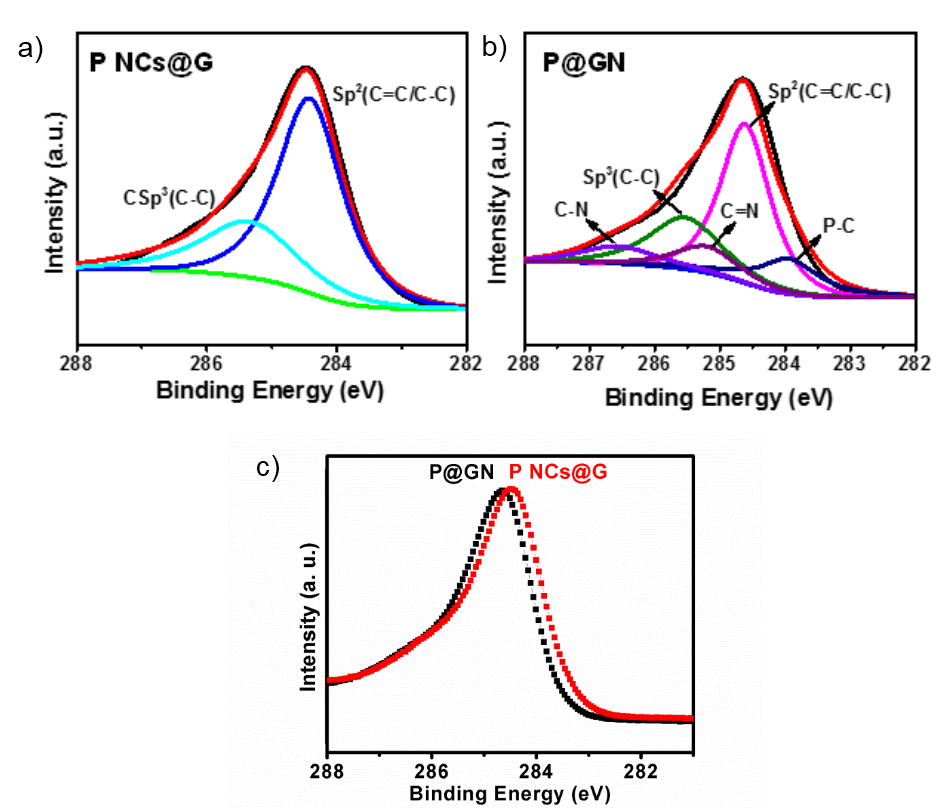
\includegraphics[width=320pt]{figures/figure4_s5}
\caption[C1s XPS spectra comparison]
{a-b) C1s XPS spectra of PNCs@G and P@GN samples. c) Overlay overlay of the two surveys for C1s spectra of the two samples. 
\label{fig:4_s5}}
\end{figure}

The content of P in the composite was determined to be ~66\% from the thermogravimetric analysis curve (Figure \ref{fig:4_s4}). As shown in Figure \ref{fig:4_1}d, the P2p X-ray photoelectron spectroscopy (XPS) is fitted to the 2p1/2 and 2p3/2 doublets, in which two peaks at 129.75 eV (2p3/2) and 130.6 eV (2p1/2) are assigned to a possibly exited P-C structure.\cite{Jiao2014b,Niu2014b,Zhang2013b} According to theoretical calculation,\cite{Sun2014b,Claeyssens2009b} among all P-C bonding types (sp3, sp2 in plane, sp2 at edge, and sp2 in aromatic ring), the most stable one is the sp2 hybridized P-C bonds in aromatic ring due to the shortest bond length in the \pi-p* conjugation plane. As the inset image illustrates in Figure \ref{fig:4_1}e, GN can provide sp2 P-C bond at the edge and within the aromatic rings. Useful information can also be gained from C1s XPS spectra shown in Figure \ref{fig:4_s5}, the possibly existed P-C bonds are presented in P@GN. For the sake of better comparison, P nanocrystlas@pure graphene (P NCs@G) sample was also prepared. As it is obvious in Figure \ref{fig:4_s5}a, there are no P-C bonds found for P NCs@G. As compared with the cases of P NCs@G, the sp2 C atom fraction decreases while sp3 C-C (285.3 eV) bonds prevail in P@GN (Figure \ref{fig:4_s5}b) due to the generated defects. Three N-doping types exist in the present P@GN (Figure \ref{fig:4_1}e): graphitic or quaternary N (N1, 401.7 eV), pyrrolic N (N2, 400.2 eV), and pyridinic N (N3, 399.1 eV).\cite{Roth1947b,Wang2012e,Wang2014f,Wang2013i} The N2 and N3 dopants are generally believed to be located at the edges or surface "hole" defect sites.\\

\begin{figure}  
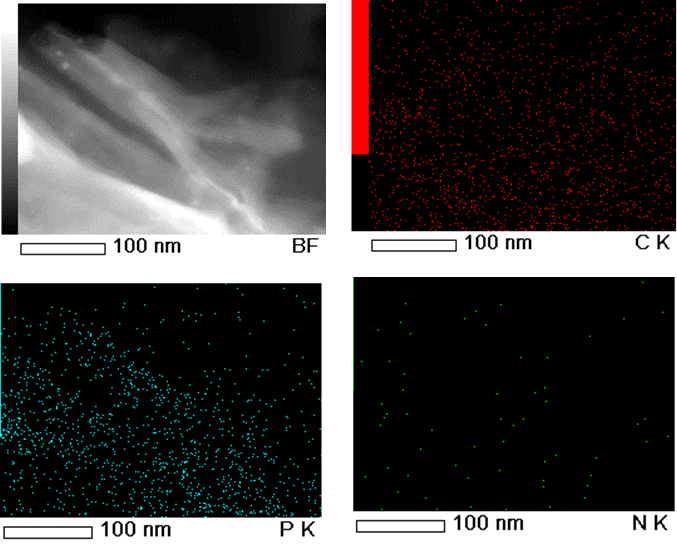
\includegraphics[width=\textwidth]{figures/figure4_s7}
\caption[Elemental maps of P@GN]
{
HAADF-STEM image, and C-, P- and N-elemental maps of a P@GN nanosheet. 
	
\label{fig:4_s7}}
\end{figure}

The designed “butter-bread”-like structure affords remarkable battery performances. As shown in Figure \ref{fig:4_2}, the electrochemical performances of the P@GN were evaluated by using standard coin cells. In order to make a better comparison, red P nanocrystals anchored on pure graphene (P NCs@G) were also fabricated by hand-grinding of nano-sized red phosphorus and graphene. As illustrated by Figure \ref{fig:4_2}a, the initial Coulombic efficiency of P@GN is as high as 87\%, higher than a figure of 85\% for the reported P@C hybrid electrode.\cite{Li2013c} From the second to 120th at 200 mA/g or 350th cycle at 800 mA/g, the Coulombic efficiencies are > 98\%. A discharge plateau in Figure \ref{fig:4_2}b corresponds to an anodic peak emerged from 0 V to 0.5 V, suggesting the formation of Na3P with the theoretical capacity of 2596 mAh/g. The conversion reaction of P → Na3P takes place, which is also proved by in situ HRTEM experiments discussed in the following sections. In the reversed scan, a main anodic peaks appears at 0.53 V, possibly corresponding to a main sodium ion de-intercalation process from Na3P to P; while no obvious peaks at other potentials (e.g. 0.63V assigned to NaP) found indicate that such electrode may experience a reversible discharging/charging between Na3P and P and holds super-high capacity due to existence of Na3P. \\



\begin{figure}  
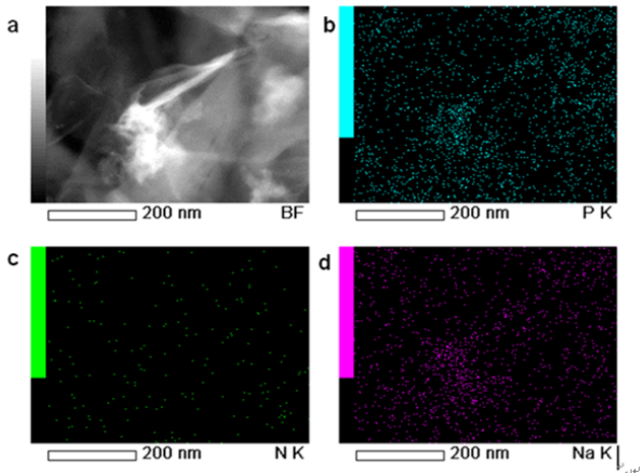
\includegraphics[width=\textwidth]{figures/figure4_s8}
\caption[Elemental maps of P@GN after 150 cycles]
{
The HAADF-STEM image and the corresponding elemental maps of a P@GN nanosheet at the fully desodiated state after 150 cycles.
	
\label{fig:4_s8}}
\end{figure}

Over 350 cycles, the capacity decay of P@GN is less than 15\%. From the 2nd to 350th cycle at 200 mA/g, the capacity retention is more than 97\%. The ultrahigh capacity retention and cyclic stability (0.002\% decay per cycle) are among the best cycling performances of all P-based anodes reported to date. To disclose the origins of such extra stable performance, the fresh and cycled P@GN electrodes have been studied by a high angular annual dark field (HAADF)-scanning TEM (STEM) technique and the corresponding elemental mapping (Figure \ref{fig:4_2}c, Figure \ref{fig:4_s7} and Figure \ref{fig:4_s8}). One can see that the integrity of the nanosheet structure is well maintained in the fully desodiated states even after 120 cycles. It is also concluded that upon sodiation the distribution of Na species is homogeneous over the nanosheet (Figure \ref{fig:4_2}c), this indicates the successful intercalation of Na ions. The volume changes of P layers are largely buffered and confined among GN layers, preventing the anode structural failure. In addition, P@GN electrode exhibits improved rate capability, as compared with P NCs@G (Figure \ref{fig:4_2}d). At a high current rate of 1500 mA/g, the reversible capacity can still reach 809 mAh/g for P@GN; this value is twice higher than the theoretical capacity of commercial graphite (370 mAh/g) in LIBs. And these results are far better than those of the P NCs@G (~10 mAh/g at 1500 mA/g). \\

\begin{figure}  
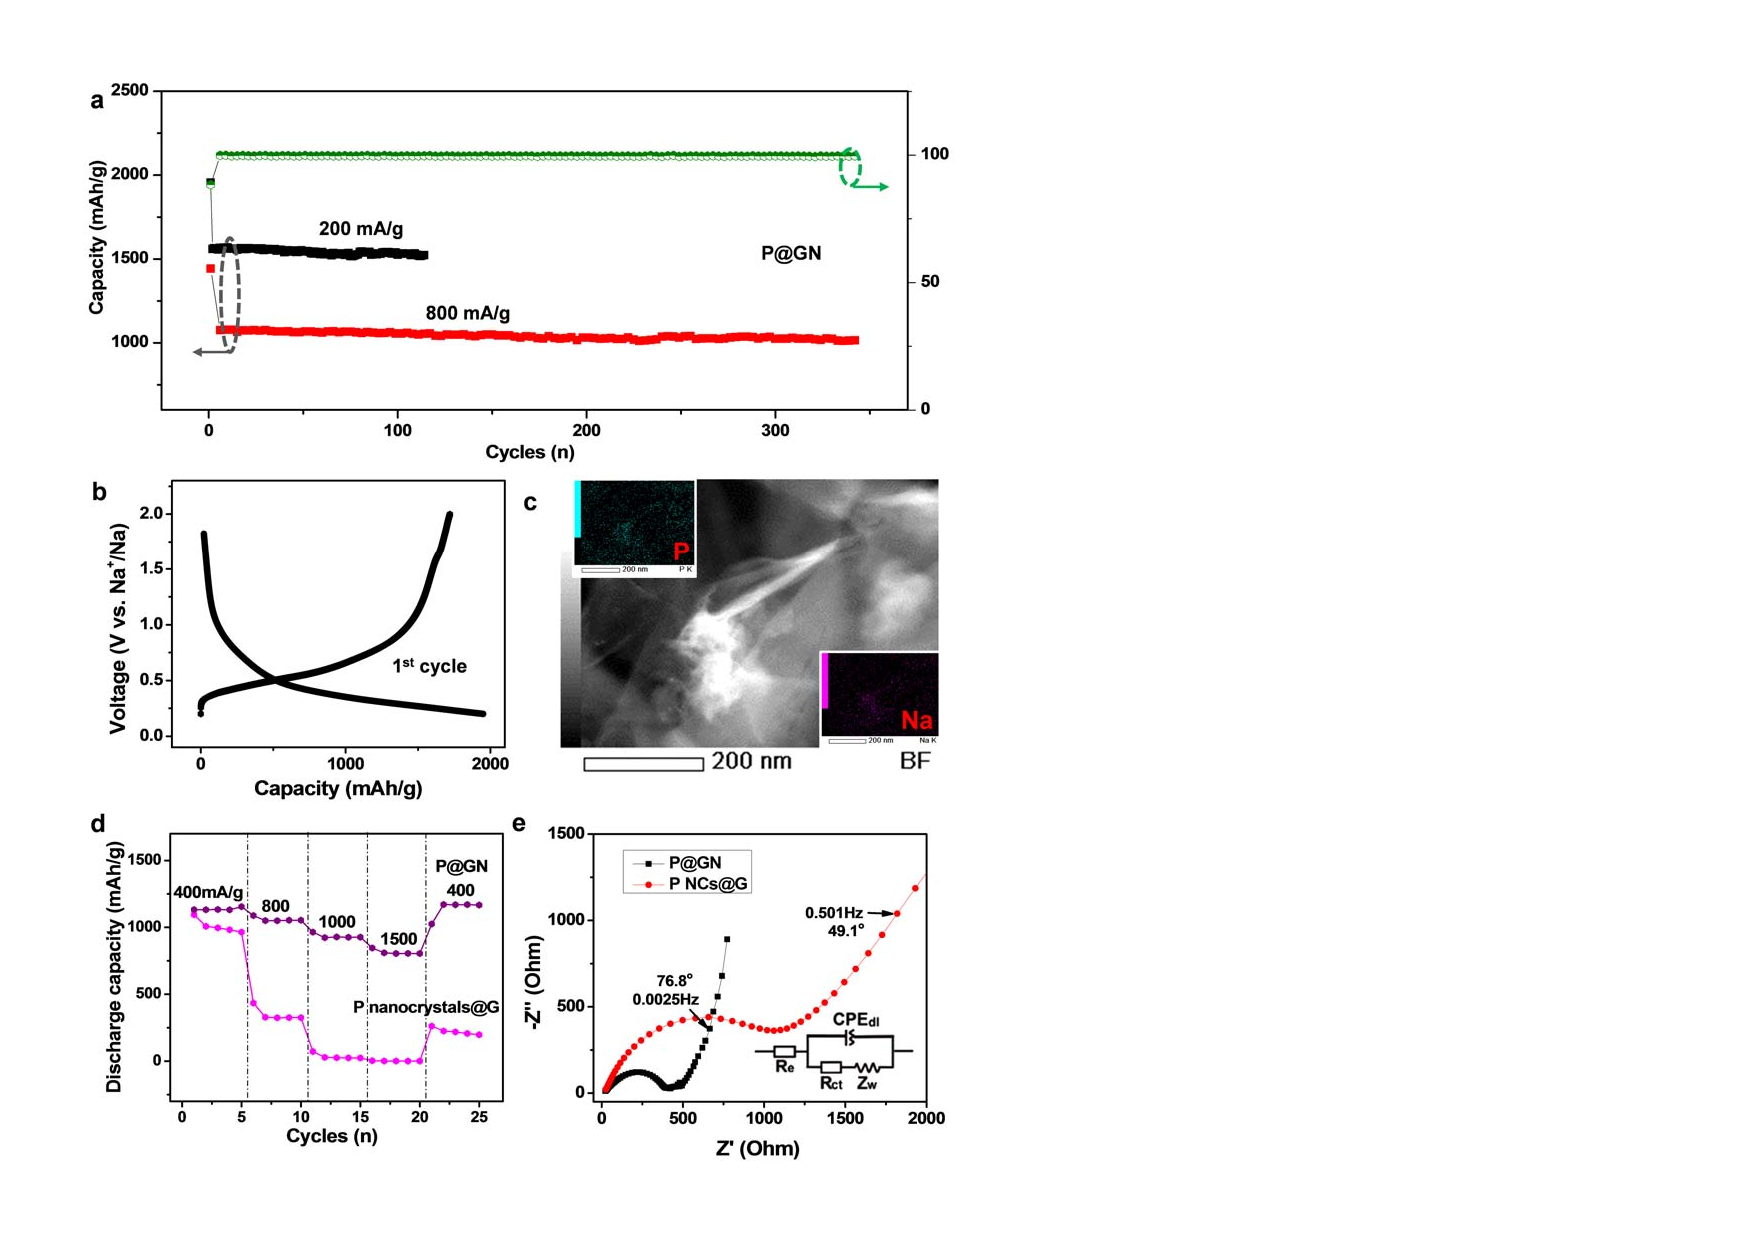
\includegraphics[width=400pt,angle=-90]{figures/figure4_2}
\caption[Performance of P@GN SIB]
{
(a) Cyclic performance and Coulombic efficiency of P@GN at 200 mA/g and 800 mA/g. (b) Galvanostatic charge/discharge profile of a P@GN electrode at 200 mA/g. (c) The HAADF-STEM image and the corresponding elemental maps (insets) of a P@GN nanosheet at the fully desodiated state after 120 cycles. (d) Comparative rate capability of P@GN and P nanocrystals@G (P NCs@G). (e) Nyquist plots and equivalent circuit model of P@GN and P NCs@G electrodes after 10 cycles at 0.1 A/g in the discharged state. All the specific capacities were calculated based on the weight of composites. 
	
\label{fig:4_2}}
\end{figure}

In order to compare the electrode kinetics of P@GN and P NCs@G, their electrochemical impedance spectroscopy (EIS) was performed (Figure \ref{fig:4_2}e). The Nyquist plots demonstrate that a diameter of the semicircle for P@GN electrode in high-medium frequency region is much smaller than that of P NCs@G electrode, thus suggesting that P@GN electrode possesses the lower contact and charge-transfer impedances. Based on the modified Randles equivalent circuit, shown in the inset of Figure \ref{fig:4_2}e, the P@GN electrode exhibits a much lower charge-transfer resistance, Rct than the P NCs@G composite electrode does (122.8 vs 279.4 Ω). It suggests that the P@GN holds a high electrical conductivity and creates a more stable surface film (including SEI layer), resulting in the better rate capability and higher reversible capacity in comparison with P NCs@G. In addition, the low-frequency slope angle for P@GN is steeper than that of P NCs@G (76.8° vs 49.1°), indicating higher Na+ ions diffusivity and good \ce{Na+} diffusivity (for Na uptake and extraction) in P@GN electrode due to the steeper low-frequency tail.\cite{Sun2014b} \\

\begin{figure}  
\centering
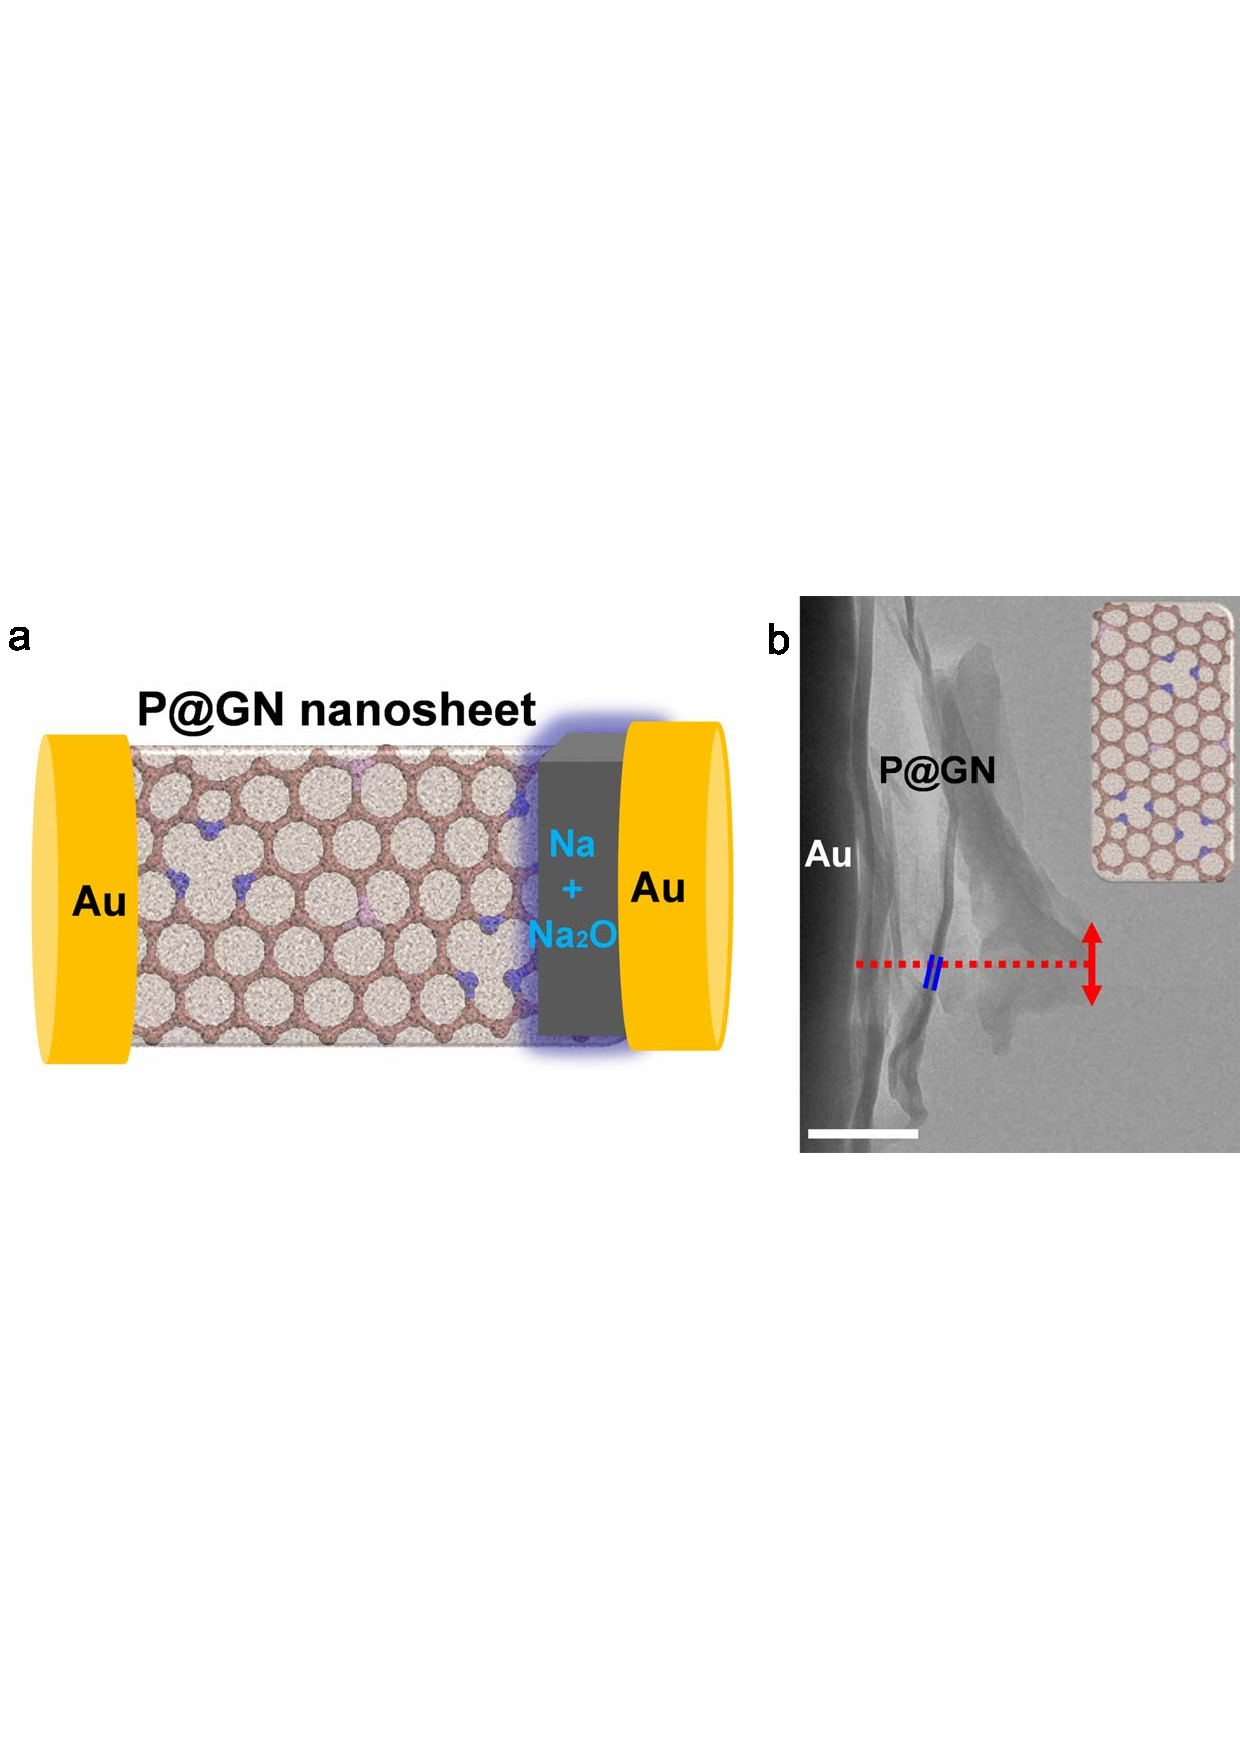
\includegraphics[width=300pt,angle=0]{figures/figure4_3ab}
\caption[{\em in situ} probing on P@GN SIB setup]
{
(a) Schematic illustration of an individual P@GN nanosheet prototype sodium battery device by {\em in situ} TEM sodiation. (b) TEM image of the nano-SIB at initial stage. Inset shows the corresponding schematic atomic structures. Scale bars: 100 nm.
\label{fig:4_3ab}}
\end{figure}

It is essential to maintain the structural integrity during cycling in order to achieve a superb cycling stability for the large-volume-change anode.\cite{Liu2014a} To clarify this point, we performed a direct in situ HRTEM study of the structural changes of the as-made anodes during sodiation (Figure \ref{fig:4_3ab}). The in situ HRTEM set-up was similar to that utilized in our previous works (Figure \ref{fig:4_3ab}a).\cite{Wang2014f,Wang2012g} This consists of two parts: an Au wire decorated with the P@NG nanosheet and another Au wire with a small piece of Na attached to its tip. During a transferring process of the material to a TEM holder, a thin layer of Na2O was formed on the Na metal surfaces, which serves as a natural solid electrolyte for the nanoscale SIB cell.4 Figure \ref{fig:4_3ab}b shows the TEM image of a freestanding pristine P@GN nanosheet. 

\begin{figure}  
\centering
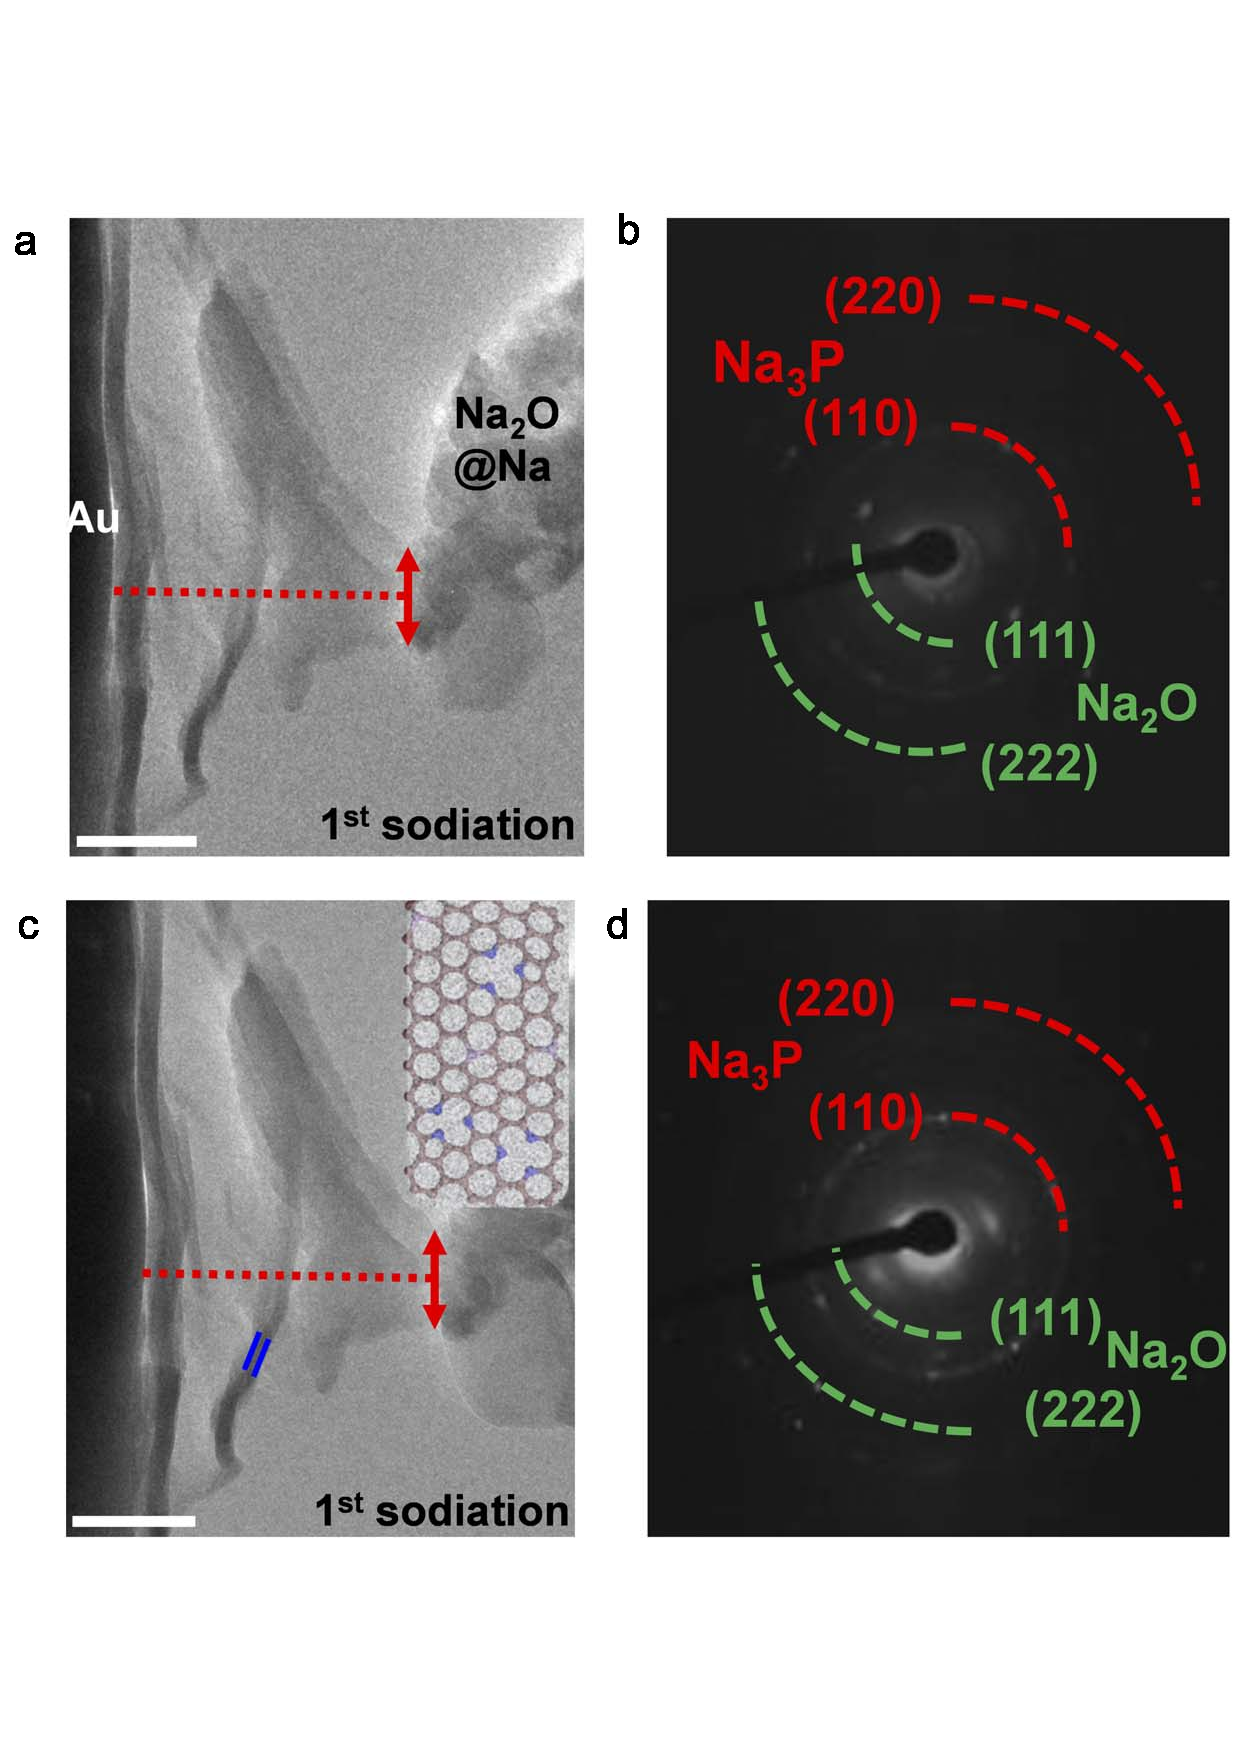
\includegraphics[width=320pt,angle=0]{figures/figure4_3cd}
\caption[{\em in situ} sodiation process of P@GN SIB]
{
 TEM image of the nano-SIB at (a) 15 s and (b) 120 s of time-lapse TEM images and selected area electron diffraction (SAED) patterns of sodiation during 1st discharging. Scale bars: 100 nm.
\label{fig:4_3cd}}
\end{figure}

Figure \ref{fig:4_3cd} illustrates the sodiation process of an individual P@GN. When a potential of -2 V was applied to the P@GN with respect to the Na metal, the nanosheet had immediately expanded along both longitudinal and transverse directions (Figures \ref{fig:4_3cd}). After sodiation, the length of nanosheet changes from the initial 210 nm to 250 nm, and the length of a small edge becomes 83 nm compared to a pristine value of 65 nm. It further demonstrates that an effective sodium transport along and across the hybrid sheets has really been taken place. Note that the elongation rate in the longer direction (210 nm to 250 nm) becomes much smaller than that for a shorter one (65 nm to 83 nm), which indicates that small-sized nanoribbons have higher electrochemical activities. There is no trace of structural degradation observed even after entire sodiation (Figure \ref{fig:4_3cd}b), confirming the superb flexibility of GN and amorphous P layer that can effectively buffer a large volume expansion during Na-insertion. The nanosheet thickness increases (10 nm → 14 nm), as marked by blue lines (Figures 3b, 3d), during the discharging process. The Selected Area Electron Diffraction (SAED) patterns of the sodiated P@GN (Figure \ref{fig:4_3cd}) provide the detailed information on phase changes after Na-insertion. The main phase in the sodiated products was identified to be Na3P, which is consistent with the electrochemical test in a real cell (Figure \ref{fig:4_2}b). 

\begin{figure}  
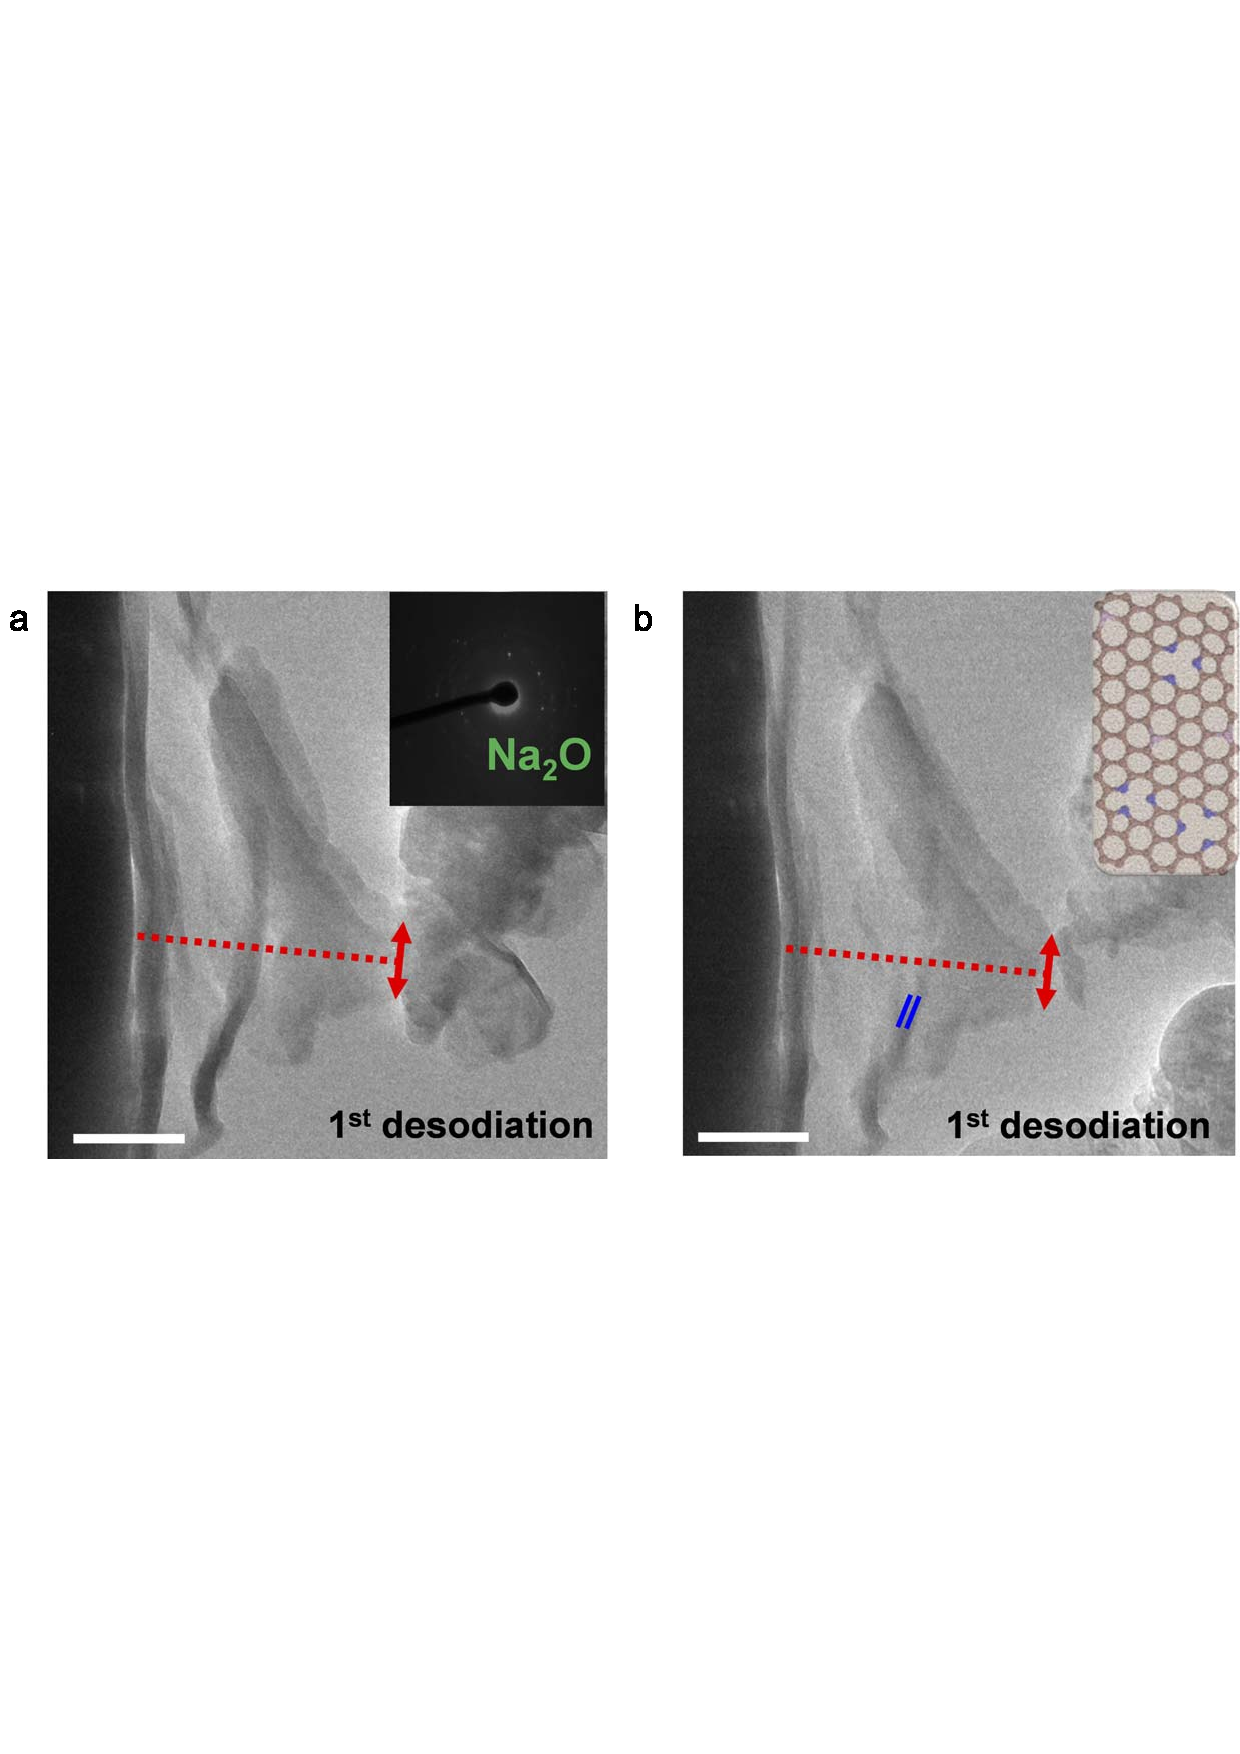
\includegraphics[width=\textwidth,angle=0]{figures/figure4_3ef}
\caption[{\em in situ} desodiation process on P@GN SIB]
{
  (a) 5 s and (b) 120 s of time-dependent TEM images of desodiation during 1st charging. Insets show the corresponding schematic atomic structures. The inset in (a) depicts the corresponding SAED pattern. Scale bars: 100 nm.
\label{fig:4_3ef}}
\end{figure}

When a potential of 2 V had been applied to the nanosheet, the desodiation process occurred. As shown in Figure \ref{fig:4_3ef}, the shrinkage becomes observable along both longitudinal and transverse directions. Note that desodiated nanosheet after Na-extraction looks nearly similar to its initial shape, in particular, the edge segment perfectly resembles the pristine state. This demonstrates that such “butter-bread”-like structure can indeed effectively buffer the volume expansion/shrinkage during discharging/charging, which explains its very stable cycling performance during the {\em ex situ} battery tests (Figure \ref{fig:4_2}b). The integrity of P@GN nanosheet is well preserved, suggesting that layered structure can indeed relax the strain, overcome the problem of pulverization, and thus serve as the promising anode candidate.\\

As a comparison, an individual P NCs@G nanosheet Na-ion battery was also built and tested in situ (Figure \ref{fig:4_s3}a). Upon discharging, the P nanocrystals expanded immediately (Figure \ref{fig:4_s3}b-d). Very different from P@GN, the whole nanosheet drastically shrinks instead of expanding upon Na-insertion along both longitudinal and transverse directions. This is because the sodiated crystals aggregated together and grew larger due to Ostwald ripening, thus the large adhesive force between G nanosheet and P nanocrystals drove the whole structure into a small aggregate under expansion of P NCs. Note that this phenomenon is much easy to be seen at the edge than on the basal plane, consistent with the higher electrochemical activities of the former. In addition, active material peeling can also be observed in this process, as revealed by blue arrows (Figure \ref{fig:4_s3}, c to d), in which two nanocrystals in the upper part and one particle in the lower part are missed during Na-insertion. This implies that the P NCs@G after Na-insertion can experience a severe irreversible expansion and peeling off, thus leading to a high capacity loss. In addition, there are some NaP phases (SAED, Figures \ref{fig:4_3cd} found in the desodiated products, demonstrating that only partial conversion of P into NaP (corresponds to 856 mAh/g) but not to Na3P (corresponds to 2569 mAh/g) takes place. The partial sodiation of P in these P NCs@G composites may be mainly associated with their poor electrical conductivity and large size of crystallites. The above-discussed issues (the irreversible structural changes and the presence of NaP) should undoubtedly deteriorate the performance for P NCs@G. This is consistent with the measured cycling and rate properties (Figure \ref{fig:4_2}c). \\

\begin{figure}  
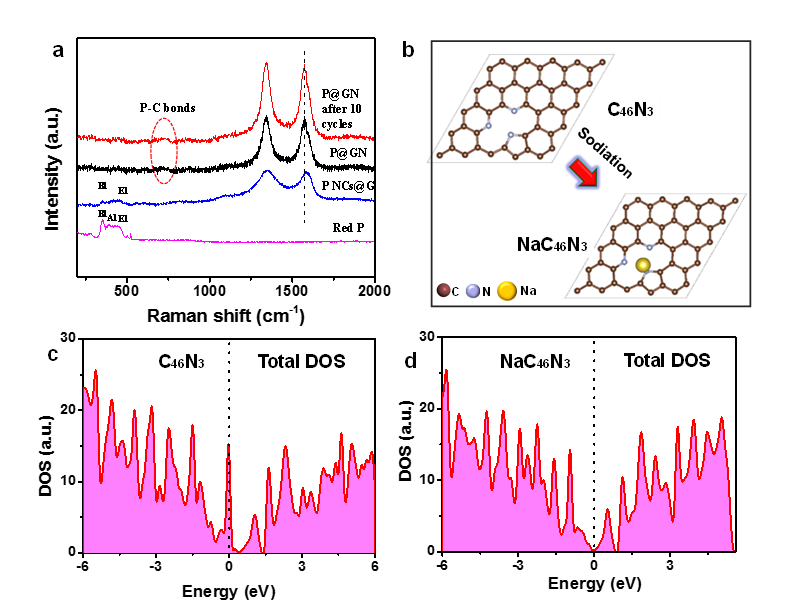
\includegraphics[width=\textwidth]{figures/figure4_4}
\caption[Raman spectra and DFT calculations]
{
(a) Raman spectra of pure red P, P nanocrystals@G, and amorphous P@GN before and after sodiation. Features of the spectrum of red P between 300-500 cm-1 can be attributed to P–P stretching bands of P9 and P7 cages arranged to form pentagonal tubes in paired layers. (b) The schematic illustration of the process of Na-insertion into a piece of N-doped graphene (C46N3) sheet based on DFT calculations. (c-d) The total calculated density of states (DOS) of C46N3 and its sodiated product \ce{NaC46N3} based on DFT calculations.
\label{fig:4_4}}
\end{figure}

In addition, maintaining the amorphous architecture of P and the existence of stable P-C bonds during multiple discharging/charging cycles is believed to be one of key factors for ultrastable cycling performance. This was further confirmed by the Raman spectroscopy (Figure \ref{fig:4_4}a). Compared with the red P powder, the present amorphous red phosphorus/graphene hybrid samples (before and after cycling) exhibited no Raman peaks natural for phosphorus; only two typical D- and G- band peaks peculiar to graphene were observed.\cite{Kim2013c} This indicates that a “butter-bread” P@GN paper consisting of amorphous P layers on the GN nanosheets’ was was well preserved during cycling. In addition, Raman spectra of various samples gave an additional evidence of the existence of stable P-C bonds after multiple cycles. As shown in Figure \ref{fig:4_4}a, a broad envelope centered at about $700 cm^-1$ for P@GN (marked as a red circle) is assigned to P-C bond stretching modes. After cycling, a stable P-C bond may exists, as depicted in Figure \ref{fig:4_4}a. The formation of coherent P-C bonds in the P@GN paper affords high capacity and cycling stability during the battery performance. In comparison, no broad peaks exist in P NCs@G and pure red P. Furthermore, compared with P NCs@G, P@GN reveals the G band shifted to a lower wavenumber ($1571 cm^-1$) due to the \pi-p* conjugation, further indicating that the formation of P-C bonds may take place. \\
Finally, DFT calculations were performed to elucidate the role of N-doped graphene on the improvement of electrochemical performances of SIBs. There have been many reports on doped graphenes (GD) utilized as LIB and SIB anode materials.\cite{Yang2011c,Wen2014b,Wang2013h,Wang2012e,Wang2014f} Firstly, we calculated the adsorption energy of a Na ion on different graphene structures. For pristine graphene and graphitic (N1)-doped graphene, this value is positive (e.g. +0.50 eV for G). It demonstrates that both pure and N1-doped graphene make the Na adsorption energetically unfavorable, that is, these two structures deliver no capacity. In contrast, for other doping forms, such as N2-/N3-doping and P-doping, it becomes negative, making them very attractive anode candidates. Herein three types of doped graphene were taken into account; the corresponding Na absorption configurations on the GN surfaces are shown in Figure \ref{fig:4_4}b. Then we obtained their corresponding capacities based on the calculation of the maximum Na concentration. Pure graphene(G) does not have charge transfer, and hence the calculated capacity is idealy 0; while C46N3(GN) present 0.851 e charge transfer, and the calculated capacity is 373.3 mAh/g, which is 1.2 times of the capacity of hard carbon (300 mAh/g) in SIBs, suggesting that N- and P-doped graphenes can contribute to capacity in addition to their positive roles in electron transport. Furthermore, the above-mentioned three kinds of doped graphenes exhibited a relatively larger charge transfer from Na, for example, Na donates 0.853|e| charge to graphene in C46N3. This further suggests that doping sites can have high efficiency to enhance the interaction between Na and graphene surface, leading to ultrafast sodium storage. The high rate capability of the doped graphene was also supported by the density of states calculations (Figures \ref{fig:4_4}c-d). For instance, doping with nitrogen makes C46N3 metallic. Above all, from the theoretical point of view, N-doped graphene is favorable for fast electron/ion transfer, superior rate capability, high capacity, and long cycling life for SIBs.

\section{Conclusions}
In summary, we designed a "phase-transformation" route to fabricate a doped graphene-phosphorous structures with layered morphologies in which very thin amorphous red P layers are formed within flexible and conductive N-doped graphene frameworks. Advantages of such SIB anode designs have been proved experimentally, they are namely: \\
(1) By spreading amorphous P to form a thin P layer on the doped graphene instead of crystalline P nanoparticles, the P@GN anode shows ultrastable efficiency (0.002\% decay per cycle from 2nd to 350th cycle) and excellent rate capability (809 mAh/g at 1500 mA/g); \\
(2) The expected P-C chemical bonds are detected, which firmly anchor GN and P layers; \\
(3) In situ HRTEM experiments on a prototype P@GN-based nanobattery device further verified its ultrastable performance and high capacity of P@GN entirely sustained during sodiation.\\
Finally, DFT calculations reveal that doping sites can enhance the interactions between Na and graphene surface, leading to ultrafast sodium energy storage. Our work demonstrates that the designed flexible amorphous P@N-doped graphene structure prepared from a "phase-transformation" approach can greatly improve the cycling and rate performances for future sodium storage. 



